\documentclass[11pt,letterpaper]{article}
\usepackage[top=1.00in, bottom=1.0in, left=1in, right=1.25in]{geometry}
\usepackage{graphicx}
\usepackage{latexsym,amssymb,epsf}
\usepackage{epstopdf}

\usepackage{sectsty,setspace,natbib}
\usepackage{float}
\usepackage{latexsym}
\usepackage{hyperref} 
\usepackage{hyperref}
\usepackage{epsfig}
\usepackage{graphicx}
\usepackage{amsmath}
\usepackage{array}
\usepackage{lineno}

\usepackage{todonotes}
\usepackage{framed}

\linespread{1.1} % was 1.66 for double-spaced 
% \raggedright
\setlength{\parindent}{0.5in}
\pagestyle{empty}

\parskip=5pt
\pagenumbering{arabic}
\pagestyle{plain}
\setlength\parindent{0pt}

\begin{document}
\begin{flushright}
Version dated: \today
\end{flushright}
\bigskip
\noindent RH: Environmental tracking 
% put in your own RH (running head)
\bigskip
\medskip
\begin{center}
% Insert your title:
\noindent{\Large {\bf How environmental tracking shapes communities in stationary \& non-stationary systems}}\\
% Other titles: `Environmental tracking: It's more complicated than you think' (we hope) 
% or `Environmental tracking: Is it naive? Or, are we just naive?'
\bigskip
\noindent {\normalsize
Lizzie$^{1}$ \& Megan$^{2}$ }\\
\noindent {\small \it
% $^1$ Arnold Arboretum of Harvard University, 1300 Centre Street, Boston, Massachusetts, 02131, USA\\
% $^2$ Organismic \& Evolutionary Biology, Harvard University, 26 Oxford Street, Cambridge, Massachusetts, 02138, USA\\
$^1$ Forest \& Conservation Sciences, Faculty of Forestry, University of British Columbia, 2424 Main Mall, Vancouver, BC V6T 1Z4\\
$^2$ Hawaii Institute of Marine Biology}\\
\medskip
\end{center}
\noindent{\bf Corresponding author:} XX, see $^{1,2}$ above ; E-mail:.\\

\newpage
%\linenumbers

% SEE ALSO: genoutline label in VarEnv_notes ... this reviews the three environmental variables. Decide how much of that we want to cover here... Maybe much of this could go in a box in the paper?

\begin{abstract} \emph{Super dry, but better to have something ... I think.} Predicting community shifts with climate change requires fundamental appreciation of the mechanisms that govern how communities assemble. Much work to date has focused on how warmer mean temperatures may affect individual species via physiology, generally producing shifts in the species' ranges and phenology and documenting high variation in the magnitude of shifts across different species, which fails to predict the wide diversity of observed shifts. This has led to a growing appreciation that improved understanding will require understanding the direct and indirect consequences of these shifts for species and their communities. Here we review how temporal variability in the environment affects species persistence in stationary environments, extending theory to understand how a species' ability to track the environment may affect their long-term persistence in communities. We then discuss how non-stationary environments may fundamentally alter these conclusions with a focus on how climate change has altered the start of the growing season. Finally we review how the reality that change has and is expected to affect far more than mean temperatures, including widespread affects on growing season length, variability and shifts in extreme events may complicate simple predictions of winners and losers with climate change. 
\end{abstract}
\noindent \emph{Keywords:} phenology, climate change....\\

% Framing: 

% Work examining how this variation may link to fitness consequences has found a positive relationship between how much a species shifts its phenology with warming with how much its fitness also changes alongside warming---such that species that shift more generally perform better with warming. 

%% TO DO (in addition to notes from lab meeting)
% (1) Get some data on the SOS changing: SOS paper from Ault group?
% (2) Get some pheno-tracking data ... 
% (3) Get some snowpack data? 
% (4) Understanding figures ... I think the tauI trade-off with R* come in early, before we introduce tracking ... can we help them make sense there?



\section{Main text}
Anthropogenic climate change is causing widespread changes in species, with many species shifting in both time and space \citep{IPCC:2014sm}. Reports often focus on species shifting to higher elevations and poleward \citep{Chen2011}, and/or shifting earlier in their recurring life history events (phenology) as climate warms \citep{Menzel:2006sq,Wolkovich:2012n,cohen2018}. A large proportion of species, however, are shifting much less \citep{Cook:2012pnas}, raising concerns about whether these species may be more vulnerable to population declines with continued warming. Such conclusions come in part from increasing research that links how well species track climate change---especially through temporal shifts---to shifts in biomass, growth and other metrics related to performance \citep{Cleland:2012}. Tracking may then be a major component to understanding and predicting indirect effects of climate change---including population declines, with cascading effects on community and ecosystem structure.

How well a species tracks the environment through its phenology has repeatedly been linked to other effects of climate change \citep{Cleland:2012,ramula2015}. Species that phenologically track warming also appear to perform better in field warming experiments \citep{Cleland:2012}, while exotic plant species appear to gain a foothold in warming environments by phenologically tracking climate change \citep{Willis:2010al}. Simple community ecology theory supports these findings, suggesting that a warming climate should open up new temporal niche space and favor species that can exploit that space \citep{gotelli1996,wolkovich:2010fee,Zettlemoyer2019}. Thus, earlier springs should favor earlier species, especially those that can environmentally track ever-earlier seasons. This hypothesis has gained significant traction in the ecological literature focused on global change \citep[e.g.,][]{Cleland:2012}, however, there has been comparatively little work examining whether it is supported through coexistence theory and models. 

Current or `modern' coexistence theory is based strongly on understanding how variable environments may promote coexistence---providing one way to study how communities may be shaped by a changing environment, and the importance of tracking. Most theory, however, is based on the assumption of stationarity: though the environment is variable, its underlying distribution is unchanged across time \citep{barabas2018}. This assumption is common not just to coexistence theory, but to much of the theory that underlies ecology, evolution and myriad other research fields \citep[e.g.,][]{nosenko2013,Milly:2008yu}. 

Climate change upends the assumption of stationarity. By causing increases in temperature, larger pulses of precipitation, increased drought, and more storms \citep{ipcc2013}, climate change has fundamentally shifted major attributes of the environment from stationary to non-stationary regimes. This transition is reshaping ecological systems, and, while new work has aimed to adapt coexistence to non-stationary environments \citep{chessonnonstat}, little work has fundamentally examined what such a transition may mean for communities and the species within them.  % Importantly, models based on the theory can help highlight which species `traits,' including those related to how species are matched to and respond to the environment, are favored under different environmental regimes.

Here we review current knowledge on temporal environmental tracking both in empirical data and though the lens of basic community ecology theory, highlighting where simple theory predicts complexities often seen in empirical results. We review current coexistence theory for variable environments, and provide an initial test of how well basic theory supports the current paradigm that climate change should favor species with environmental tracking. Finally, we provide a framework to leverage existing ecological theory to understand how tracking in stationary and non-stationary systems may shape communities, and thus help predict the indirect consequences of climate change. % We begin with an overview of coexistence theory for variable environments and what predictions models from this theory make for stationary environments. In particular, we look at how species traits related to their responses to environmental variability effect coexistence and long-term persistence in community maintenance. Using a simple example, we show how current models can be extended to non-stationary environments (similar to those due to climate change) to examine how changing environments alter predictions.

\subsection{Environmental variability \& change}

Decades of ecological research highlight how variable environments shape species and their communities at multiple scales \citep{Sale:1977oq,Chesson:1997dz}.  In much of the globe where feasible periods for growth each year are limited (e.g., by temperature or drought) species must manage within-year variability to time when to grow and when to reproduce \citep{donohue2002}. This environmental variability compounds into inter-annual variability and critically shapes the start and end of growing seasons. For long stretches of history this variability has been stationary; that is, the underlying probability distribution that produces it does not change even though one year may be dramatically different than the next. The shape of this underlying distribution varies across systems and in how it is measured---the total amount of rainfall in semi-arid systems is often highly skewed compared to the more normal distribution of the thermal sum of many temperate growing seasons.

In other time periods variability is non-stationary in one or multiple dimensions. For example, climate in the northern hemisphere includes long warming and then cooling periods (i.e., increasing then decreasing means of the probability distribution) at the start of the Holocene, when the earth was coming out of the last glacial maximum. Anthropogenic climate change (henceforth referred to simply as `climate change') is a similar non-stationary process, with warming seen around the globe and knock-on effects for other climate metrics, such as heat extremes, the size of precipitation events etc.. While only several decades ago, ecology was focused strongly on stochasticity in stationary systems \citep[e.g.,][]{Ripa1996,Kaitala1997}, climate change has shifted the focus to understanding stochasticity within a non-stationary framework \citep[e.g.,]{cazwavelets,ehrlen2016}.

Understanding non-stationarity in ecological systems requires first identifying what has shifted in the underlying distribution that produces variation in the transition from stationary to non-stationary, and what remains constant. For example, with climate change, warming has increased mean temperatures over time, with minimum temperatures generally increasing more than maximum---this results in an underlying distribution for daily temperature where the mean is increasing through time and the variance is decreasing \citep{ipcc2013,screen2014}, despite a growing literature on increasing variance in temperature \citep[e.g.,][]{vasseur2014}. [ADD another example: San Diego or Snowpack or Lake Washington?.]  % Many current ecological models then provide a pathway to understand how such transitions may impact communities. 

% Recent advances in coexistence theory, often heralded under the title `modern coexistence theory,' recognize that both mechanisms independent of fluctuations in the environment (e.g., R* and other classical niche differences) and dependent on fluctuations in the environment (relative non-linearity and storage effect) can drive coexistence \citep{Chesson:1997dz}. Models under this paradigm are thus often composed of parameters the describe the environment and the species within it (Megan--suggestcitations). Parameters related to species must always include mechanisms for growth, death, interactions with other species, and generally a bet-hedging strategy for survival across years (e.g., a seedbank or other long-lived lifestage)---though exactly how these are defined varies across models (e.g., R* and related models focus on resource competition). How the environment is defined in most models falls into two broad categories. In some models the environment is expressed as variation in parameters related to species (e.g., in some lottery models the environment appears, effectively, as variation in birth and death rates). In other models, the environment is more specifically defined. For example, many seed germination models define an environment that begins with a resource pulse each year. Building a changing environment into models thus may require knowing how environmental shifts filter through to species-level parameters \citep{Tuljapurkar2009} or---perhaps more simply---how the environment is changing. In the aforementioned seed germination models, many systems may be experiencing shifts in the size or variability of the resource pulse.
% \citep{Davison2010,morris2008,Tuljapurkar2009}
% Lottery model: Birth and death rates vary ... collapses to single ratio (that's the environment) ... many general models are like this, they just vary a parameter and assume it is varying in response to the environment. Whatever parameter you allow to vary is how you allow the environment to filter through. (Side note: Tulja Purqur may have worked on how environment filters through to many species parameters in the model.)

\subsection{Environmental tracking in time}
% Review Phillimore paper (photoperiod x temperature)?
% Review crazy Iler paper (detrending)?

Environmental variability, and the reality that it is often well described by some underlying probability distribution, means most species should benefit from tracking their environment. We focus here on environmental tracking through time (often referred to below as `tracking') rather than through space because of its well-established links to individual-level physiology, yielding a more robust understanding of what environmental cues determine tracking \citep{chuineJTB,Chew:2012pd}, and because it has been repeatedly linked to performance and other fitness-related metrics. Temporal environmental cues, however, are often linked to species' ranges \citep{Morin:2008vp,arabid2011}, thus we expect much of this work could extend to environmental tracking through space.  % especially given a better understanding of it through time. 

% Environmental variability, and the reality that it is often well described by some underlying probability distribution, means most species should benefit from tracking their environment through time---most often through adjusting their phenologies.
Many species track their environments through time by adjusting their phenologies, but identifying this tracking depends on many factors. Defining---or measuring---environmental tracking depends on the level of the question, and how well researchers understand a species' underlying physiology and ecology. Many, or all species, for example use abiotic cues to trigger major phenological events (e.g., leafout in trees or emergence of insects each spring). Tracking may thus often be defined simply by the relationship between the dates of the phenological event and a simple abiotic metric, such as a relevant mean monthly temperature, with variation in temperature derived from multiple periods of observation or induced through experiments. 

Simple environmental metrics are almost always proxies for a more complicated underlying physiology where simple cues---such as those to warm temperatures---can be modified by other cues, such as photoperiod, drought or light spectra \citep{Bagnall1993,Stinchcombe:2004ec}. These additional cues almost always appear designed to handle unusual---though not completely uncommon---years when the simple cue alone would fail, that is trigger growth, reproduction or another life history event at a highly suboptimal time. For example, in many temperate forest systems, woody plants cue strongly to warm spring temperatures, but also to cool winter temperatures, which prevents leafout in warm snaps that occur in many climates in the middle of the winter---long before the last risk of frost damage is past. In some semi-arid systems, species time growth to pulses of rain, but only when those rain events occur with cooler temperatures, that indicate the start of the rainy season, and not a rare summer rainfall event in the middle of months of drought.  % Process-based models can help include some of these complexities, especially when informed by observational and experimental results, but even for such well studied systems as \emph{Arabidopsis thaliana} there is still some noise in predictions versus empirical results. 

%  All these approaches  are focused on the proximate level---what environmental cues underlie tracking---at the ultimate level tracking is shaped by what resources species need to grow and reproduce. 
The complexities of cues underlying environmental tracking highlight that, at the ultimate level, tracking is shaped by complex resources that species need to grow and reproduce. This is perhaps best recognized in the literature on trophic synchrony where focus is often on how well consumers track their prey resources \citep{deacy2018, kharouba2018}. For example, decades of work has studied how birds (e.g., \emph{Parus major}) time their peak food demands---during their nesting season---to caterpillar (their prey) abundance \citep[e.g.,][]{charm2008}. Failure to track prey year-to-year or over time with warming has been well tied to individual-level fitness consequences in some systems \citep[e.g.,][]{charm2008}., but not all \citep{visser2006}. Tracking of plants and other lower trophic levels is also equally about resources. Alpine plant species that emerge in step with snowmelt are likely responding, at least in part, to light resources for photosynthesis. Light equally appears critical to the sequence of phenology in many temperate forests: with lower-canopy species, and younger (shorter) individuals of higher-canopy species, routinely risking frost damage to leafout before the canopy closes and access to light becomes severely reduced \citep{Vitasse2013,heberling2019}. In both temperate as well as alpine systems, however, access to critical belowground resources also occurs in the spring---both for available water but also for nutrients released at the turnover of the microbial communities \citep{Zak:1990ar}. Thus, plants' spring phenology in many systems is about careful tracking to optimally compete for nitrogen and other soil resources. As in higher trophic level systems, research has linked how well plants track to performance, with species that track warming better tending to grow larger and/or produce more offspring \citep{Cleland:2012}.
% Hetherington or such paper that I reviewed for light and canopy?
% Ref for variation in tracking among consumer species (linked to fitness)?

% ADD  some numbers on variation in tracking ... why the variation? (1) it's hard to measure (keep this quick? Reference box?) and (2) maybe it's not always optimal to track ... boom, coexistence theory to the rescue!
Variation in metrics of tracking highlights that---despite the clear importance of tracking for resource access---not all species appear to track their environments equally well. Some temperate woody species track spring temperatures strongly (give some examples), but other species do not (NUMBERS) and do not appear linked to other major climate variables (CITES). Variability equally exists when examining consumers tracking their prey (NUMBERS). Such variation in tracking across taxa is driven in part by difficulties in measuring tracking (see BOX). Yet other variation may be real, and suggests perfect environmental tracking may either not be possible or optimal for all species. 

Ecological theory predicts variation in tracking across species for multiple reasons. First, how predictable an environment is affects how much species can track. Tracking is only beneficial to species---and possible---when the environment is predictable. Predictability depends on the timescale of interest, which is related to a species' generation time \citep[which itself should be shaped by an environment and its predictability,][]{Davison2010,morris2008}. Species with longer generation times may track low frequency climate signals and make investment choices on far longer timescales than species with shorter lifespans \citep{morris2008}. Perhaps unsurpisingly tracking appears best studied in some of the most predictable environments and at the most predictable timescales; for example much research examines how temperate trees track the annual start of the temperate growing season, which always corresponds to temperature increasing and daylength lengthening. Inter-annual events such as extremely good or poor years for reproduction may be more difficult in some systems to predict, and thus there is little potential to track. In such cases, species should gain a substantial benefit from bet-hedging or employing other approaches that spread out risk given uncertainty \citep{Venable:2007os,donald2013}. Even in highly predictable environments, evolutionary limitations may prevent perfect tracking: species may not be able to closely measure relevant environmental cues \citep{arnold1992,Singer:2010eb}, gene flow from other other environments may continually push a population away from its local optimum \citep{lenormand2002}, or there may be unavoidable trade-offs \citep{levins1968} with tracking. 

Within populations, life-history can help predict how much individuals should track while also balancing trade-offs within and across seasons and years. Tracking has been repeatedly linked to fitness benefits \citep[e.g.,][]{farzan2018,deacy2018}. Such benefits usually break down into avoiding tissue loss or maximizing growth and, relatedly, maximizing reproduction. Species often track the start of growing seasons to avoid substantial tissue loss, for example from frost damage in temperate plants, or start activity only when resources for growth are present, such is the case in animals coming out of hibernation in cold regions. Equally, tracking of resources throughout a season is linked to the timing of reproduction for many species and, for iteroparous species, decisions on how much to invest each season requires estimating how likely a year is to be good for offspring. For species with bounded growing seasons, much literature has reviewed how tracking is a multivariate equation balancing early-season access to resources and its associated risks of tissue loss, with later season tracking of resources for reproduction and time for offspring to mature \citep{donohue2002,Morin:2005ye,Burghardt2015}. These trade-offs should also scale up to predictions of variation in tracking across species. 

Across species, community ecology theory makes predictions for suites of traits that may trade-off with tracking. As tracking fundamentally relates to tracking a resource pulse in most systems, traits related to resource use are likely contenders for a trade-off. Species with traits that make them poor resource competitors may need to track the environment closely, while superior competitors could outcompete trackers, and thus hypothetically track the environment less closely. Examples include under-canopy species leafing out earlier to gain access to light or plants with shallow roots starting growth sooner in semi-arid systems, while species with deeper roots may begin growth later. In such cases, tracking is akin to a competition-colonization trade-off \citep{Amarasekare:2003tq}, where species that track well gain priority access to resources, and thus may co-exist with superior competitors. [Here we add a short lit review showing that people have found this? Or not ... or not looked.]
% ii. Links to trait literature? Not enough study of traits that include tracking components (because that’s hard)
%      A. how much do people look at trade-offs?
%      B. phenology can impact traits themselves, so how to analyse (competition experiments?)

Trade-offs with tracking, predicted by basic ecological theory and supported by growing empirical work, would have fundamental consequences for community assembly, especially with climate change. Applying this ecological theory to current environments, however, is difficult because most theory has been developed for stationary systems \citep[as is the case in other sciences also, ][]{Milly:2008yu}, which are mathematically more tractable, and can sometimes be extended to non-stationary systems \citep{chessonnonstat}. Almost no community assembly research, however, has examined the consequences of shifting from a stationary to non-stationary environment. Yet this transition is exactly what anthropogenic climate change has imposed on systems around the globe, making our understanding of how environmental tracking fits within community assembly theory critical. 
% .... that would have fundamental consequences for community assembly---at least in stationary systems. In non-stationary systems, theory is less developed for how tracking may trade-off with other traits (CITECHESSON), and even less theory predicts the consequences if the environment shifts from stationary to non-stationary

% How to explain warming experiments where researchers have identified links between performance and tracking, 
% links between tracking and performance in warming experiments could potentially wash out over longer timescales (fitness not measured over long enough timescales to consider diverse species life history strategies)

% consider cost of static timing (cheap) versus tracking (potentially costly)
% Variation in tracking may also be predicted based on historical effects ... change in environment (species track old environment)

\subsection{Coexistence theory \& environmental tracking (or) The role of the environment in coexistence} 
Recent advances in coexistence models, often heralded under the title ‘modern coexistence theory,' recognize that both mechanisms independent of fluctuations in the environment (e.g., R* and other classical niche differences) and dependent on fluctuations in the environment (relative non-linearity and storage effect) can drive coexistence \citep{Chesson:1997dz,Chesson:2000vd}. Models under this new paradigm are thus often composed of parameters the describe the environment and the species within it (Megan--suggest CITES). Parameters related to species must always include mechanisms for growth, death, interactions with other species, and generally a bet-hedging strategy for survival across years (e.g., a seedbank or other long-lived lifestage)---though exactly how these are defined varies across models (e.g., R* and related models focus on resource competition). 

How the environment is defined in most models falls into two broad categories. In some models the environment is expressed as variation in parameters related to species (e.g., in some lottery models the environment appears, effectively, as variation in birth and death rates). In other models, the environment is more specifically defined. For example, many seed germination models define an environment that begins with a resource pulse each year. Building a changing environment into models thus may require knowing how environmental shifts filter through to species-level parameters \citep{Tuljapurkar2009} or---perhaps more simply---how the environment is changing. In the aforementioned seed germination models, many systems may be experiencing shifts in the size or variability of the resource pulse. 
% \citep{Davison2010,morris2008,Tuljapurkar2009}
% Lottery model: Birth and death rates vary ... collapses to single ratio (that's the environment) ... many general models are like this, they just vary a parameter and assume it is varying in response to the environment. Whatever parameter you allow to vary is how you allow the environment to filter through. (Side note: Tulja Purqur may have worked on how environment filters through to many species parameters in the model.)

These models, which underlie much of current community ecology research \citep{Mayfield:2010fe,barabas2018,ellner2019}, allow tests of basic predictions of how tracking may shape communities. While growing empirical research supports that tracking is an important trait---especially in a changing environment---there are few tests of whether models support these basic theoretical predictions. Below we examine how tracking may shape communities in stationary environments and environments transitioning from stationary to non-stationary.

\subsubsection{Model description}
% To understand the role of environmental tracking by species in variable environments 
We use a simple model that includes dynamics at both the intra-annual and inter-annual scales. As the model is akin to many commonly used seed germination models \citep{Chesson:2004eo}, we follow a similar terminology for ease, however the basic structure of our model could apply to others systems with one dominant pulse of a limiting resource each season (e.g., water from rain or snowpack).  This model thus allows within- and between-year dynamics to contribute to coexistence. Between-years the environment is included via variable germination, and within-years the environment is explicitly included as a resource pulse at the start of the season. The model includes a suite of species traits, including some relating to how species respond to the environment via germination each year and some related to how species may bet-hedge across years (via a seedbank), as well as traits relating to resource competition each year. Within-season dynamics within the model thus allow for fluctuation-independent coexistence (e.g., trade-offs in resource competition), while interannual variation in the environment provides opportunities for coexistence via fluctuation-dependent mechanisms. 
% Megan says: Because there is seedbank for survivorship from year to year it allows for a storage effect mechanism of coexistence and there are fluctuation-dependent and fluctuation-independent ($c_i$) mechanisms ...

% Conceptualization of our germination equations in other file ... Megan says we could equally assume tauI means 'I go at the same time each year and the timing of the water varies ...' ... Peter's version and this give the same answer. But we need to make clear that directionality doesn't matter -- lower tauI does not germinate before higher tauI, no sequences here! ... everyone germinates at the same time in the model!

Across years, for a community of \(n\) species, the seedbank ($N$) of species $i$ at time $t$ is determined by the combination of the survival ($s_i$) of the fraction of seeds that did not germinate that season ($1-g_{i}(t)$) plus new biomass ($B_i$) produced during the length of the  growing season ($\delta$) converted to seeds ($\phi_i$):
\begin{align}
N_{i}(t+1) & =
s_{i}(N_{i}(t)(1-g_{i}(t))+\phi_{i}B(t+\delta)
\end{align}
The production of new biomass each season follows a basic R* competition model: new biomass production depends on its resource uptake ($f_i(R)$ converted into biomass at rate $c_i$) less maintenance costs ($m_i$), with uptake controlled by $a_i$ and $u_i$:
\begin{align}
\frac{\partial B_{i}}{\partial t} &  = [c_{i}f_{i}(R) - m_{i}]B_{i} \\
f_{i}(R) & = \frac{a_{i}R^{\theta_{i}}}{1+a_{i}u_{i}R^{\theta_{i}}}
\end{align}
With the initial condition:
\begin{align}
B(t+0) & = N_{i}(t)g_{i}(t)b_{0,i}
\end{align}
The resource ($R$) itself declines across a growing season due to uptake by all species and abiotic loss ($\epsilon$):
\begin{align}
\frac{\mathrm{d}R}{\mathrm{d}t} & = - \sum_{i=1}^{n}f_{i}(R)B_{i} -\epsilon R
\end{align}
Each year the proportion of seeds that germinate depends on both each species and the environment that year. The faction of seeds germinating each year for a species is determined by the distance between $\tau_i$, a species characteristic, and $\tau_P$, an attribute of the environment, which varies year to year. Germination fraction declines according to a Gaussian distribution as the distance between $\tau_i$ and $\tau_P$ grows (we refer to this distribution as the `germination curve').
% We conceptualize the distribution from which $\tau_P$ is drawn as the underlying probability distribution that drives variation in the environmental trigger for germination. 
% tauI in non-tracking is fixed characteristic of when I germinate ... and my success each year is about how far off I was. 

The model is designed for multiple conceptualizations \citep{Chesson:2004eo}, but given our focus here we consider $\tau_P$ to represent the environmental (abiotic) start of the growing season each year, and refer to it as the `environmental start time' while $\tau_i$ represents the intrinsic biological start time for species $i$ which we refer to as `intrinsic biological start time'. How well matched a species is to its environment each year can be measured as $\tau_i$-$\tau_P$, or the distance between the intrinsic (biological) start time and the environmental start time.
% tauI - intrinsic (biological) start time (bioSOS)
% tauP - environmental start time (envSOS) 
% tauIP - distance (synchrony) from environmental start time or SOS (versus biological start time)
\begin{align}
g_{i} & = g_{max,i}e^{-h(\tau_{p}-\tau_{i})^2} 
\end{align}
\noindent \emph{Adding phenological tracking to model:}\\
% tauI as fixed versus flexible or fixed versus tracking
$\tau_i$ can be considered a fixed characteristic of a species or it may respond to the environment dynamically through what we refer to as environmental tracking. Tracking ($\alpha$, which can vary between 0 to 1) decreases the distance between $\tau_i$ and $\tau_P$ such that a species with higher tracking  will have a higher germination fraction.
% maybe use SOS to abstract more ... the model is about timing, and is about the beginning of something asynchronous to something else ... should we use synchrony? 
\begin{align*}
\alpha & \in 0 \rightarrow 1  
\end{align*}
\begin{align}
\hat{\tau_{i}} & = \alpha \tau_{p} + (1-\alpha)\tau_{i}
\end{align}
\noindent Thus:
\begin{align*}
\text{when } \alpha = 0: & \hat{\tau_{i}}=\tau_{i}\\
\text{when }  \alpha = 1: & \hat{\tau_{i}}=\tau_{p}
\end{align*}
We refer to $\hat{\tau_{i}}$ as `effective biological start time' for species $i$ (or `effective $\tau_i$'). 

As our interest is primarily in the role of environmental tracking we focus on situations where species vary in their match to the environment (through both tracking, $\alpha$, or a more fixed response, $\tau_i$) or their resource uptake (via $c_i$). For simplicity, we focus on two-species communities.

\subsubsection{Tracking in stationary environments}
Species occurring for long periods of time in any habitat must be sufficiently matched to their environment across years. In our model this means species must have a germination curve such that their effective biological start time ($\hat{\tau_{i}}$) is sufficiently close to the environmental start time ($\tau_{p}$) to allow germination of new seeds before the seedbank is exhausted. In our model this can happen in two ways: species with fixed intrinsic biological start time ($\tau_i$) values close enough to the environmental start time ($\tau_P$ ) or species with a combination of intrinsic biological start time ($\tau_i$) and tracking ($\alpha$) that brings the effective biological start time ($\hat{\tau_{i}}$) close enough to the environmental start time ($\tau_P$).
% Notation version of the above: In our model this means species must have germination curves [define above?] such that their $\hat{\tau_{i}}$ is sufficiently close to $\tau_{p}$ to allow germination of new seeds before the seedbank is exhausted. In our model this can happen in two ways: species' with fixed $\tau_i$ values close enough to  $\tau_{p}$ or species with combination of $\tau_i$ and tracking ($\alpha$) that brings the $\hat{\tau_{i}}$ close enough to  $\tau_P$.

% Add histogram here with tauI and tauP and alpha! Conceptual FIGURE: stationary environment and you can get a certain distance from that mean tauP via two ways: tracking or tauI. 

A simple outcome of this model is that in temporally variable environments where all other species characteristics are identical the species with the effective biological start time closest to the average environmental start time will always win---regardless of whether this effective biological start is due to a fixed intrinsic start time or due to tracking. Put another way, in a stationary environment both tracking and a fixed intrinsic start time are equally useful ways to match to the environment---all that matters is the effective distance between the biological and environmental start of the season. This is because both represent the same niche axis---the temporal niche. 
% NEED A FIGURE FOR THIS!
% {\bf Are these effectively the same trait (so no trade-off possible)?} Right, NO trade-off possible, but it's not so much that they are the same trait, but they are trading off on the same species-response to the environment. ... things that we conceptualize as two different traits in a biological sense are the same mathematically (biologically you can imagine a trade-off between tracking and fixed tauI (and in a broader fitness model, you could put energy in either place), but in this environmental space they both get you to the same space). It's the same niche axis!

As both a fixed intrinsic start time and tracking represent the same major niche axis species cannot coexist given only variation in these traits---coexistence requires variation in another trait axis. As discussed above, many commonly cited traits for this trade-off revolve around traits related closely to resource competition \citep{Chesson:2004eo}. With this added variation---here we varied species' $R^*$ (via $c_i$)---species can persist together as long as those species with a temporal niche advantage are also the inferior competitors (FIGS). That is, species that can draw resources down to a lower level and are thus the superior resource competitors (lower $R^*$) can persist with species with that are inferior competitors given those species have higher tracking values or fixed intrinsic start times close to the most common timing of the resource pulse (i.e., species with the superior biological start times). These trade-offs, however, are all environmentally dependent. They hold only so long as the environment is stationary. 

\subsubsection{Tracking in non-stationary environments}
% Skipping -- for now -- what happens in one-species communities with no trade-offs 
A shifting environment may fundamentally reshape trade-offs that structure communities. Modern coexistence theory is based mainly on variable, but stationary, environments. As systems shift from stationary to non-stationary the trade-offs on which some communities are based may be transformed. Using our simple germination model we shifted the environment of our two-species communities---that otherwise had experienced a variable but stationary environment---to an earlier start of season by shifting the mean XX over XX years (see Supp). By changing a fundamental niche axis---on which these communities were structured---we shifted one major part of the trade-off axis: the new non-stationary environment favored an earlier effective biological start time than the previous stationary environment. This in turn reshaped communities in both our simulations built on species with fixed intrinsic start times and with start times that varied via tracking. 

In communities where species traded off competitive traits ($R^*$) with a fixed intrinsic biological start time trait ($\tau_i$), species with earlier start times were clearly favored, generally driving the other species (with a lower $R^*$ and later start time) locally extinct before the end of our XX year time-period. Very few two-species communities persisted through the end of the non-stationary period (2 out of 547 two-species communities persisting after end of stationary, or 0.04\%) and those that did were generally persisting via being highly similar---having nearly identical $R^*$ and fixed intrinsic biological start time traits ($\tau_i$). These species were persisting through equalizing mechanisms---by being almost the same neither species could drive the other extinct, though these species do not coexist (as in longer simulations through drift or related mechanisms one species would be lost). The contrast of equalizing mechanisms---stabilizing mechanisms---include niche differences such as the trade-off in competitive traits ($R^*$) with a fixed intrinsic biological start time trait ($\tau_i$). Yet, in this non-stationary system stabilizing mechanisms failed to yield any persistence of two-species communities as the environment shifted away from the previous trade-off axis the communities formed in. 
% tauI x R* runs: 2 two-species pairs left after non-stat out of 547 two-species pairs left after stat (34100 total runs), overall total species at end of stat: 10728 and end of non-stat: 298

Persistence of two-species communities via both stabilizing and equalizing mechanisms occurred more often in communities where species traded off competitive traits ($R^*$) with tracking ($\alpha$). While again, the non-stationary environment favored higher trackers, who in turn drove the extinction of species with lower tracking values from many two-species communities, some two-species communities persisted (257 out of 1698 two-species communities persisting after end of stationary, or 15.1\%). These communities included equalized species, as well as [insert more understanding here.] Taken together, this simple simulations show how non-stationarity can drive local species extinction and reshape the underlying assembly mechanisms of communities. These results however make many assumptions, including how they model non-stationarity in the environment. 
% alpha x R* runs: 257 two-species pairs left after non-stat out of 1698 two-species pairs left after stat (29600 total runs), overall species at end of stat: 26529, and end of non-stat: 1703

Our models impose environmental non-stationarity on an axis fundamental to co-existence. Other results would be expected depending on whether that non-stationary reshapes a fundamental niche axes involved in the trade-off. Non-stationarity in the environment can take on many forms---in what variable it effects and how it reshapes the underlying distribution. Communities that assemble via other axes of the environment than start of season timing may be far less impacted than our simulations suggest. Further, we examined a common trend with climate change---shifts in the mean of the environment. Changes can also occur in the variance or the fundamental shape of the distribution (e.g., shifting from a normal distribution to one that is more similar to a gamma). Additionally, we applied a shift to only one aspect of the environment. In reality climate change may impose multivariate shifts.

\emph{Multivariate nonstationary environments}\\
Human modification of climate, the nitrogen cycle and habitat impose complex shifts in the environments of most species. If the environment is altering multiple niche axes---along which species assemble---it may allow trade-offs that structure communities to persist through non-stationary periods. We examined this possibility by again shifting the mean start of season XX earlier over XX years at the same time that we shifted the size of the resource pulse lower (XX over XX years). Thus, our environment favored species with earlier start time and superior competitive abilities (given the decreasing resource). We found little evidence, however, of communities persisting via a maintained trade-off---instead the inherent variability of a system shifting in two dimensions drove species extirpations more slightly quickly (14.8\% of two-species communities remaining after non-stationary). Thus, while theoretically multivariate nonstationary environments could maintain trade-offs, the shifts would need to be so balanced that it seems unlikely. More likely appears the possibility that myriad shifts in the environment make species more vulnerable to local extirpation \citep{sixthectinction2011,IPCC:2014sm}.
% alpha x R* runs with R0: 225 two-species pairs left after non-stat out of 1521 two-species pairs left after stat (29900 total runs), overall species at end of stat: 27373, and end of non-stat: 1498


\subsubsection{Future research in environmental tracking \& non-stationary systems}
As we have reviewed, growing empirical research highlights that environmental tracking is linked to species performance, and thus may be critical to understanding the forces that assemble communities---especially as anthropogenic climate change is reshaping the environment of all species. Indeed, research in this area has often been focused on understanding the impacts of climate change, and comparatively less often been guided by testing or developing ecological theory. Current models of coexistence, however, are clearly primed for understanding how the environment can shape the formation and persistence of communities. Yet modeling efforts need more focus on understanding the attributes of an environment shaped strongly by humans, and thus, what advances in theory may be most useful and applicable in modern ecology. To this aim, we review several major questions that we believe could most rapidly unite empirical and theoretical research in environmental tracking to advance the field.\\

\emph{How is the environment changing?} \\ % Which abiotic aspects of the environment are changing? How are they shifting?

Climate change has shifted the environment of all species, often in multivariate ways. Most systems are seeing increases in mean temperatures, which can rapidly impact the metabolism and reshape of activity periods of many species \citep{Monson:2006vt,IPCC:2014sm}. This warming is also altering many other attributes of the climate system, including altered precipitation regimes in many systems \citep{Diffenbaugh2015}, and shifts in cloud cover \citep{hofer2017}, which can all further influence species. 

While we focused on one major shift in the climate system (earlier growing seasons), much more research is needed to understand how other singular shifts in the environment impact the assembly dynamics of communities in current models; and to layer on how multivariate environmental shifts may alter these predictions. Empirical ecologists can guide these efforts by identifying environmental shifts that are often linked (e.g., warming temperatures may drive earlier seasons and higher evaporative loss of some resources such as water). They can also aim to more consistently and fully characterize the environmental distributions of their systems that appear to most drive species performance and interactions: the environment of the years of study should be clearly reported and compared against long-term and recent climate for each system.\\

\emph{What major traits trade-off with tracking?} \\

Basic theory suggests environmental tracking must trade-off with other traits to allow multi-species communities. Yet to date empirical work has mainly documented tracking, linked it to performance, or focused on how it varies between native and non-native species \citep{Willis:2010al,wolkovichAmBot2013,Zettlemoyer2019}. Such work lays the groundwork that environmental tracking is important, but advancing empirical research should address how this trait co-occurs with other traits. Research on this has already highlighted some traits, that co-vary with tracking (CITES), but to tie this empirical work to models requires more research on traits that link clearly to theory. Traits that link to resource competition, as we focus on here, may be especially fruitful for greater research, but should not be the only ones considered. For example, traits related to predator tolerance or avoidance may also play a role, but have been effectively unstudied.  As empirical research in this area grows models can aid progress in understanding what the outcomes of these trade-offs may be for community assembly.\\ 

\emph{How do shifts to non-stationary environments re-shape the relative influence of stabilizing versus equalizing mechanisms?} \\

Our simple models showed that as environments shift from stationarity to non-stationarity species co-occurring via equalizing mechanisms can persist longer. While this is a rather obvious outcome---as equalized species will be similarly effected by environmental shifts---it has several important implications. First, it may make identifying which traits climate change promotes through stabilizing mechanisms more difficult. Second, it suggests climate change---or other factors that cause an environment to shift from stationary to non-stationary---may cause a fundamental shift away from assembly via stabilizing mechanisms, but this implication presumes communities include species co-occurring via strong equalizing mechanisms. Thus understanding the prevalence of stabilizing versus equalizing mechanisms \citep[which ecology has worked on for many decades,][]{Caswell:1976np,Gravel:2006ax,Chesson:2000vd} becomes critical for understanding the implications of transitions to non-stationary environments. 

If equalizing mechanisms are rare in natural communities then climate change could promote species loss by fundamentally re-shaping stabilizing mechanisms. This finding however assumes a closed community with no evolution. In practice, communities may lose species but also gain new species through dispersal, allowing communities to potentially adjust to new trade-offs as the environment shifts. In addition, evolution may allow some species to stay in communities they would otherwise have been lost from. But with non-stationarity this axis is constantly shifting---so continual community change via species loss, gain and reshaped species via evolution may be the expectation, until the environment shifts back to stationarity.
% All this suggests we need to better understand transitions from stationary to non-stationary environments more in ecology.

\subsection{Stationarity in the future}

While most environments today are climatically non-stationary, and have been for decades, the climate will return to stationarity in the future. There are many possible pathways to climatic stabilization in the future, but almost all require first the stabilization of greenhouse gases---the subject of much policy and political debate. Once greenhouse gas emissions stabilize climate will not quickly snap back to a new stationary phase. Instead systems will slowly approach a new climatic stationarity depending on how they are effected by the earth's multiple thermal reservoirs, and, in turn, how quickly those reservoirs stabilize. The timescale of this approach is generally expected to be on the scale of centuries, but could be much longer in certain oceanic systems \citep{ipcc2013ch12}. Thus, ecologists are---and will remain in---in a research area structured by climatic non-stationarity. 

As paleobiologists and evolutionary biologists often point out, climatic nonstationarity is a common part of the earth's history \citep{Jansson:2002nz}---even if stationary periods of cold or warm (glacial and interglacial periods) are more common. Indeed, while much of this work has examined how species survive for millions of years given dramatic climatic change \citep{provan2008}, the periods that provide the most dramatic community reshuffling---from stationary to non-stationary climate \citep{vrba1980,vrba1985}. Such stories of the past are now fundamentally happening today, and ecology is challenged to understand how transitions between stationary and non-stationary environments is reshaping the species and communities we have today and will in our warmer future. 

% START HERE! 
% (*) Keep re-reading and refining once 1-2 are started!
% (3) Check the outline and below for what to add or move to an obvious to do list!
% (4) Should probably read the Volker paper and the new Zettlemoyer (2019 ELE)

% Chapter 12 of IPCC WG1 "Long-term Climate Change: Projections, commitments and irreversibility" (Section 12.5: Climate Change Beyond 2100, Commitment, Stablizition and Irreversibility)

% Note to self: environmental tracking seems used by spatial folks ...
   % https://www.nature.com/articles/srep36265
% But! The temporal autocorrelation folks use it too ... this is mainly one-site population work I think and pretty damn similar to our use!
   % https://royalsocietypublishing.org/doi/10.1098/rspb.2011.0487 (2011)
   % https://link.springer.com/article/10.1007/s12080-015-0276-6 (2016)
   % https://besjournals.onlinelibrary.wiley.com/doi/full/10.1111/1365-2745.12077 (2013) 
% And this annual review has a whole section (no definition though that I saw):
   % https://www.annualreviews.org/doi/full/10.1146/annurev.ecolsys.35.120202.110110 ... about fossil 'The principal cause for these patterns appears to be species-, and perhaps clade-level, environmental fidelity that results in long-term tracking of physical conditions. ... biotas do appear to track climates, but such tracking is certainly influenced by geographic and physicochemical barriers' 
% So I say it is all the same thing! And we focus here on the temporal aspect .... give nod to space at the end of ms maybe?


\newpage
\section{Figures}
\begin{enumerate}
\item Figure for ... The shape of this underlying distribution varies across systems and in how it is measured---the amount of rainfall in semi-arid systems is often highly skewed compared the thermal sum of many temperate growing season
\item With climate change, warming has increased mean temperatures over time, with minimum temperatures generally increasing mre than maximum---this results in an underlying distribution for daily temperature where the mean is both increased through time and the variance is decreasing (Munich garden? Maybe add San Dieg precip example?
\item Real-world data showing stat/non-stationarity in environment (ideally $\tau_{P}$) 
\item Real-world data showing tracking (and less tracking)
\item $\tau_{i}$ vs. R* trade-off and histogram of persisting $\tau_i$ under stat/nonstat $\tau_{P}$ environment
\item alpha vs.$\tau_i$ trade-off and histogram of persisting alpha under stat/nonstat $\tau_{P}$ environment
\item alpha vs. R* trade-off and histogram of persisting alpha under stat/nonstat $\tau_{P}$ environment
\item (Scratch this one: we're pretty sure it required a crappy $\tau_i$ to survive the initial stationary period, then be favored in second time period and we're not so sure crappy $\tau_i$ species survive the initial stationary period) time-series of one run showing years where $\tau_i$ of one species is close to $\tau_{P}$ and other years where $\tau_i$ of other species is close to $\tau_{P}$ (and show this shift under nonstat)
\item non-stationarity in $R0$ and $\tau_{P}$
\end{enumerate}




%=======================================================================
% \section{}
%=======================================================================

%=======================================================================
%\section{Acknowledgements}
%=======================================================================



%=======================================================================
% References
%=======================================================================
\newpage
\bibliography{/Users/Lizzie/Documents/git/bibtex/LizzieMainMinimal}
\bibliographystyle{/Users/Lizzie/Documents/git/bibtex/styles/ecolett.bst}


%=======================================================================
% Tables
%=======================================================================

%\begin{center}  
%\begin{table}
%\caption{Key differences between PWR and traditional PCMs such as PGLS.}
%\begin{tabular}{ | p{4cm} | p{5.5 cm} | p{5.5 cm} |}   \hline 
%& PWR & PCMs (e.g., PGLS) \\ \hline \hline
%Major goal & Study of evolution of correlation between variables across species & Study of evolution of correlation between variables across species\\ \hline
%\emph{Assumption 1:} Nature of correlation between two or more variables & Non-stationary (changes through phylogeny in a phylogenetically conserved fashion) & Stationary (constant) throughout phylogeny (all variation is noise) \\ \hline
%\emph{Assumption 2:} Completeness of variables & Substitutes phylogeny for variables (simple or complex) not in the model that interact with variables in the model & Assumes variables in model are primary drivers of correlational relationship \\ \hline
%Inferential mode & Usually exploratory & Hypothesis testing (statistical significance)\\ \hline
%Outputs & Coefficients of regression changing through the phylogeny & p-value and single set of coefficients presumed to apply to entire phylogeny with their confidence intervals\\ \hline

%Method to avoid overfitting & Cross-validation (boot-strapped determination of optimal band-width for accurate prediciton of hold-outs) & Exact analytical model of errors and degrees of freedom\\ \hline \hline
%\end{tabular}
%\end{table}
%\end{center}

%=======================================================================
% Figures
%=======================================================================
\clearpage

\begin{figure}[t!]
\centering
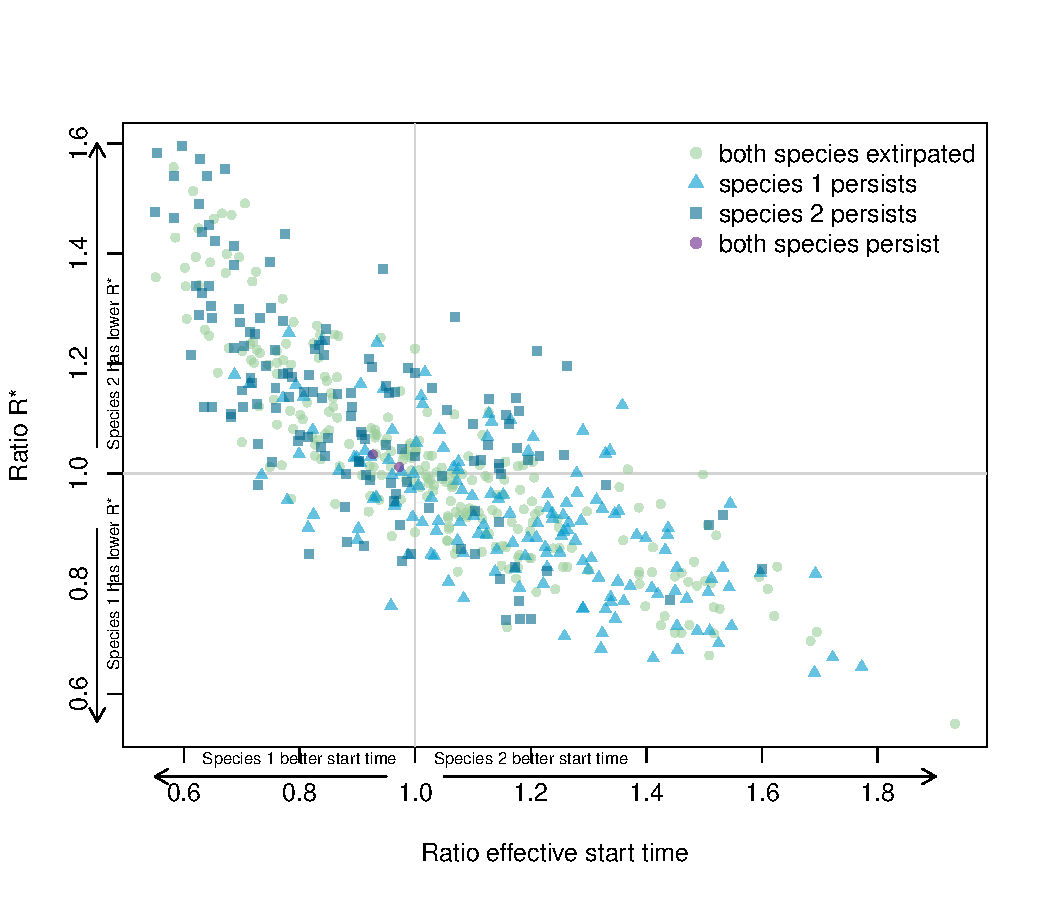
\includegraphics[width=1\textwidth]{..//..//R/graphs/modelruns/manuscript/tauIPrstart1.pdf}
\caption{Goober}
  \label{fig:tauirstar}
\end{figure}


\begin{figure}[t!]
\centering
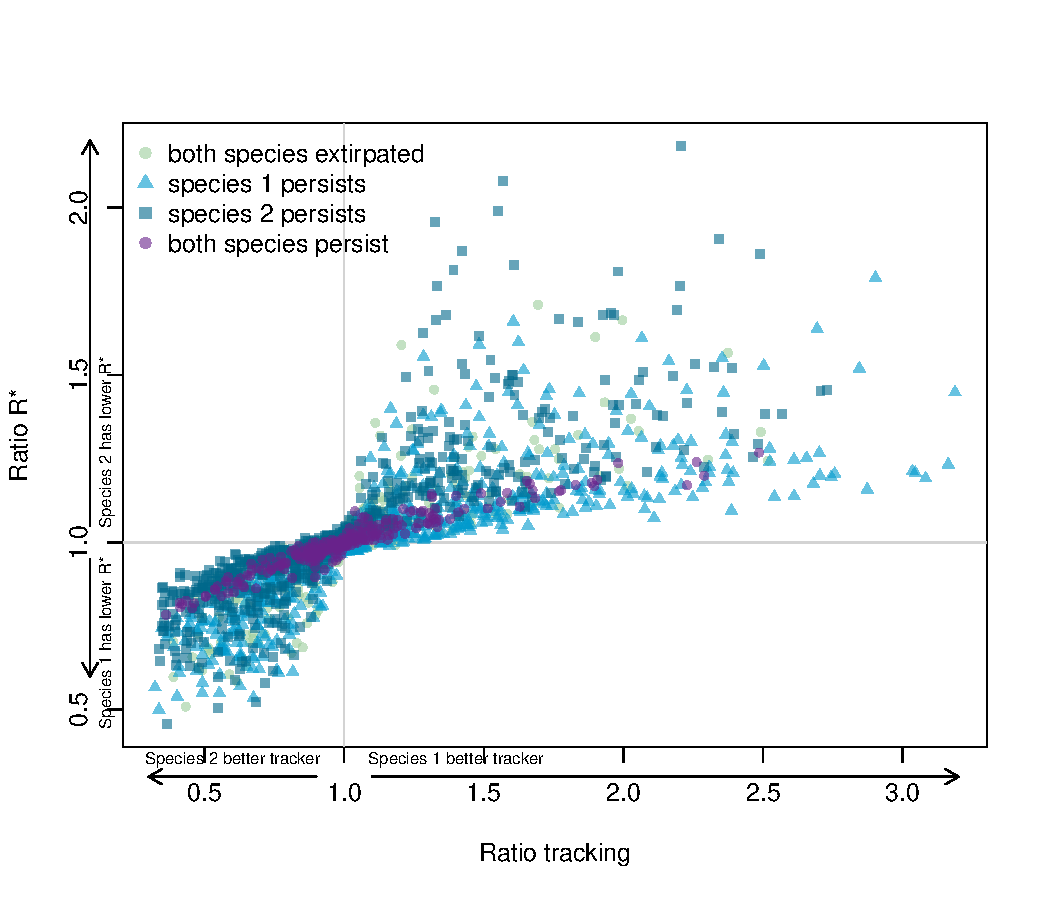
\includegraphics[width=1\textwidth]{..//..//R/graphs/modelruns/manuscript/alpharstar.pdf}
\caption{Goober}
  \label{fig:alpharstar}
\end{figure}


\end{document}
%%%%%%%%%%%%%%%%%%%%%%%%%%%%%%%%%%%%%%%%%%%%%%%%%%%%%%%%%%%%%%%%%%%%%%%%

% Example figure

\begin{figure}[t!]
\centering
\includegraphics[width=1\textwidth]{arnell-pwr-m.pdf}
\caption{PWR estimates (red dots) and 95\% confidence intervals (red lines) across the Arnell phylogeny using O-U-based distance  weighting, for a simple regression of first flowering date on seed size. Solid and dashed vertical gray lines show the estimate and 95\% CI from an analogous global model estimated using PGLS.}
  \label{fig:arnell-pwr}
\end{figure}
\clearpage


%=======================================================================
% to-do listing
%=======================================================================

\listoftodos

%=======================================================================
\section*{Other loose ends}
%=======================================================================

% Old hypothesis: Without tracking we may predict benefits to early-colonizers decline with earlier seasons. As start-date moves earlier, early folks lose benefit (assuming they tend to often go at optimum time) and you get more late folks. Late species may be less different than one another---and less responsive to environment. Early folks, effectively, become more similar to environment. 



% Old parts of intro not currently used....
Athropogenic climate change is causing widespread changes in species, with many species shifting in both time and space (CITES). Many species are shifting in ways predicted by a direct response to track climate---for example, species are shifting up in elevation and poleward as climate warms (CITES), and/or shifting earlier in their recurring life history events (phenology)(CITES). Yet, not all species are shifting as predicted by a simple climate-tracking response; species in the same community can include some that do not shift or even shift in an apparently opposing direction (e.g., delayed spring phenology with warming). \\

Understanding these variable responses of species and communities to climate shifts is a major aim of current ecology and may be explained by indirect effects. Research has already documented changes in a species performance (CITES) and community composition that appear to be---at least in part---indirect effects (CITES).  Understanding ecological responses to climate change will thus require synthesizing information on both direct effects of climate on species and indirect effects driven by responses to other species' shifts. \\ % Alongside these more direct physiological effects of climate change, however, are indirect effects.






